% !TEX root = ../main.tex
% Implementierung
In diesem Kapitel werden die genutzten Technologien vorgestellt und eine Einblick in die Realisierung der Arbeit gegeben.
Der Abschnitt \ref{subchap:app-struct} behandelt die Struktur der Applikation und geht auf die verwendeten Klassen ein, verdeutlicht durch Abbildung \ref{fig:uml-app} in einem \emph{UML}-Diagramm.
Die Klasse \emph{Model} stellte dabei das Kernelement der Applikation dar und wird ausführlicher betrachtet.
In der Klasse wird aus dem gerichteten Graph von Kategorien der Kategorienbaum konstruiert und auch die gefilterte Ähnlichkeitsmatrix der Artikelvergleiche gespeichert.
Im Abschnitt \ref{subchap:external-libs} wird ausgeführt welche Bibliotheken in der Arbeit genutzt wurden.


\section{Programm Struktur}\label{subchap:app-struct}

Die Applikation ist eine in \emph{c++} und \emph{OpenGL} realisierte Visualisierung mit verschiedenen Bibliotheken, welche in Abschnitt \ref{subchap:external-libs} weiter erläutert werden.
Für die Architektur von Applikationen aus dem Bereich der Informationsvisualisierung existieren unterschiedliche Modelle, wie z.B. die von Chi \cite{EdHuaiHsinChi}, Card \cite{card1999readings} oder Tang \cite{Tang2004}.

Die Abbildung \ref{fig:card-model}, zeigt den Aufbau des Entwrufsmusters nach Card et al. \cite{card1999readings}.


Aus der Abbildung geht hervor, dass die Elemente \emph{Model} und \emph{View} aus dem \emph{MVC}-Muster im Referenzmodell weiter in kleinere Bausteine zerlegt werden.
Der Baustein \emph{Model} wird in die Bausteine Datenquelle und Datensatz unterteilt.
Der Baustein \emph{View} wird wiederum in visuelle Struktur und Ansicht gegliedert.
Durch diese Staffelung wird zwischen Datenmodell und visuellem Modell unterschieden und dadurch eine leichtere Handhabung der... ermöglicht.
Zusätzlich bedeutet sie eine Spezifizierung des \emph{MVC}-Musters für Informationsvisualisierungen.
Die Strukturierung der Applikation in dieser Arbeit orientiert sich an dem Entwurfsmuster des Referenzmodells.
Die Abbildung \ref{fig:uml-app} zeigt ein UML-Diagramm der Applikation mit ihren Klassen.

Nach dem Referenzmodell von Card et al. \cite{card1999readings} bestehen die Rohdaten der Visualisierung sowohl aus dem Wikipediadatensatz als auch aus der Ähnlichkeitsmatrix.
Eine Umwandlung von Rohdaten in eine geordnete Struktur, wie der Objekt-Relationalen-Datenbank, wird im Modell als Datentransformation bezeichnet.
Im Abschnitt \ref{subchap:datenverarbeitung}, wird diese Transformation im Detail erklärt und durch Abbildung \ref{fig:ablauf-daten} veranschaulicht.
Die Umwandlung der Datentabellen in visuelle Repräsentanten geschieht in der Klasse \emph{Model}.
Die Klasse \emph{Model} stellt die 

Die Klasse \emph{model} aus Abbildung \ref{fig:uml-app}, stellt die visuelle Struktur dar. % siehe s. 17 reading in information visualization visual thinking.
In ihr wird sowohl der Kategorienbaum konstruiert als auch die aus der Datenbank gefilterte Ähnlichkeitsmatrix gespeichert.
Im UML-Diagramm ist zu erkennen, dass die Klasse noch weitere Funktionen hat. Hierzu gehört das Anordnen der Kategorienpositionen oder die Erweiterung des Kategorienbaums.
Die Klasse \emph{renderer} stellt dabei die Ansicht der visuellen Struktur dar. Durch diese Klasse wird die Schnittstelle zur Grafikkarte hergestellt.
Die Klasse realisiert Teilbereiche der Interaktionen, wie die Verschiebung, Vergrößerung oder die Rotation, aber auch das primitive Zeichnen der Knoten und Kanten.
Die Klassen \emph{GUI} und \emph{View} fügen der Ansicht grafische Benutzerelemente, wie die Suchleiste oder die statistischen Zusammenfassungen, als auch die Beschriftung der Kategorien mit ihren Titeln hinzu.
In Kapitel \ref{chap:visualization} wird im Detail darauf eingegangen.

% beide grafiken zu MVC und refMODEL
\begin{figure}
    \centering
    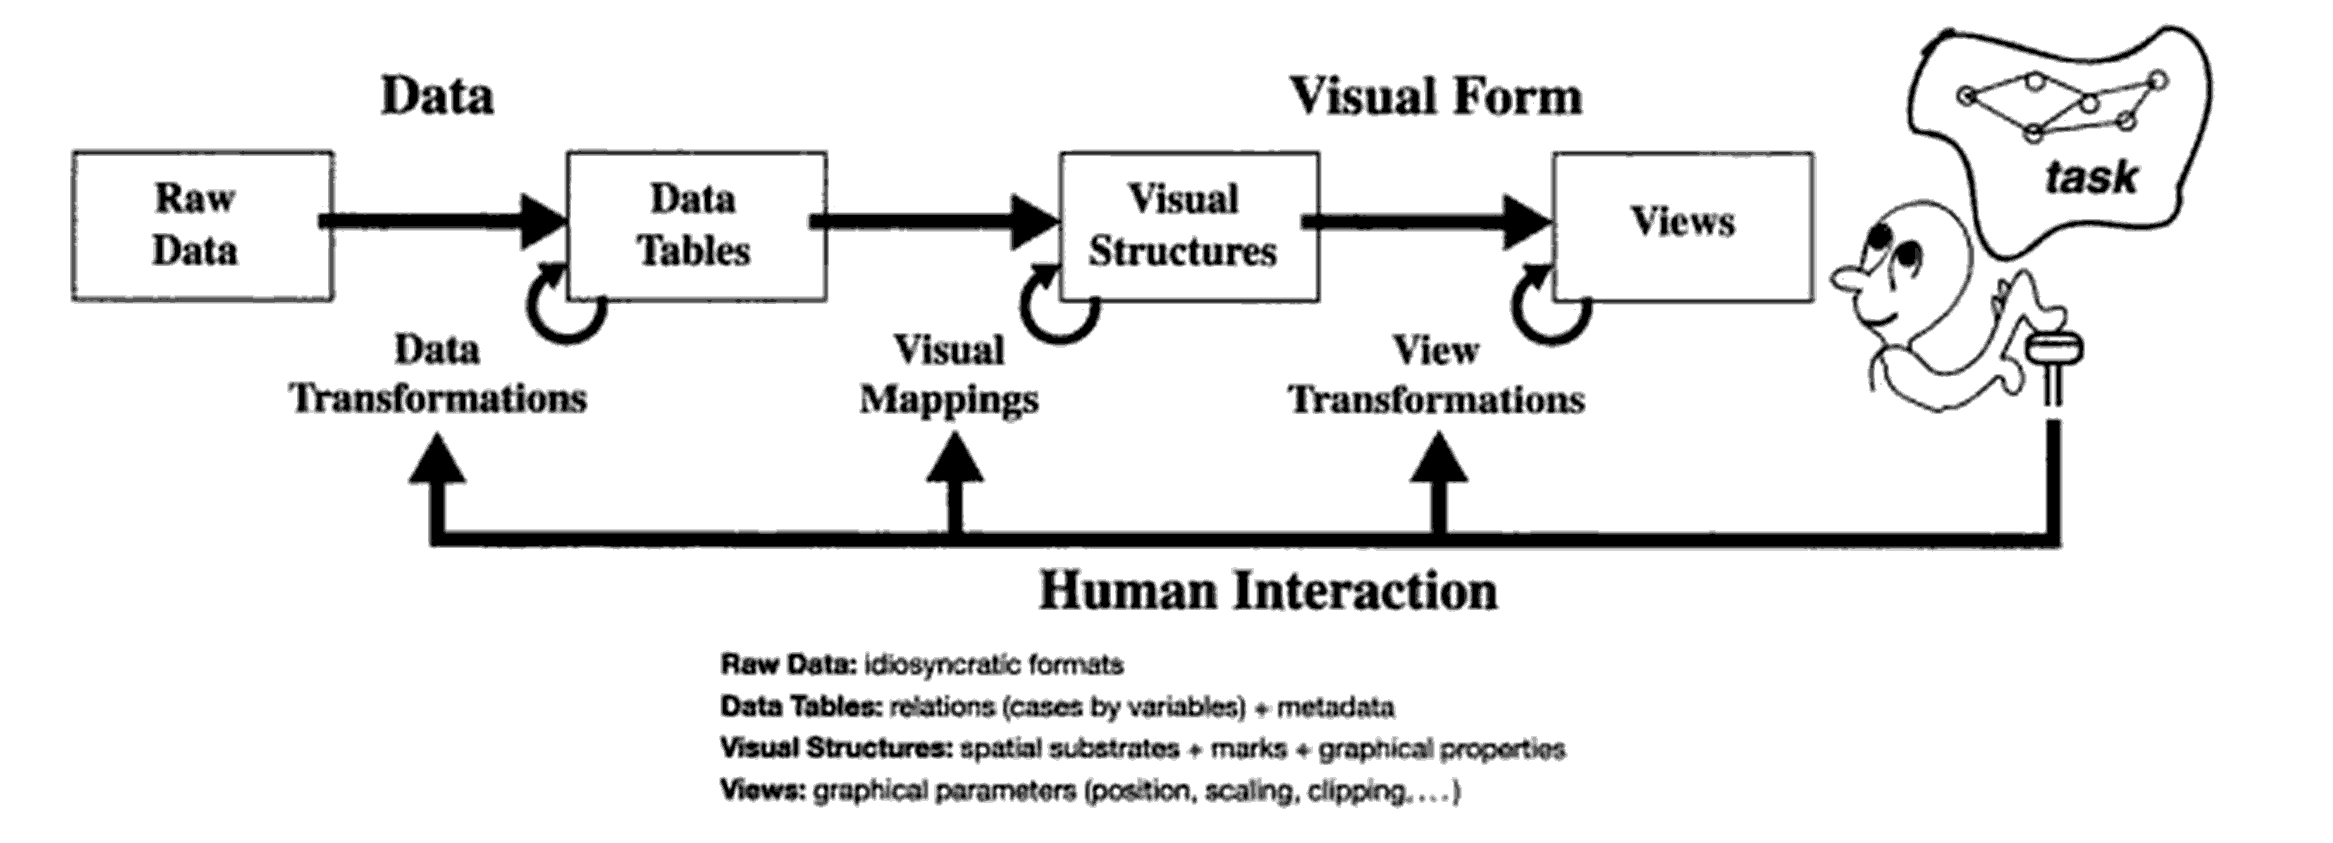
\includegraphics[width=\textwidth]{images/card-model.png}
    \caption{Referenz Modell nach }
    \label{fig:ref-model}
\end{figure}



% grafik mit schema eines Baumes und doppelten kanten zu veranschaulichung
% pseudocode!! 
\paragraph{Kernfunktionen}
Im nachfolgendem Abschnitt wird auf die Kernfunktion, die Konstruktion des Kategorienbaumes, der Klasse \emph{Model} eingegangen.
Wie bereits in Abschnitt \ref{subchap:layout} angedeutet, wird eine Methode entwickelt, welche aus den gerichteten Verknüpfungen der Kategorien, die der Datenbank entnommen werden, einen Baum konstruiert.
Die Methode muss dabei gewisse Voraussetzungen erfüllen.
Der abgeleitete Baum muss eine hierarchische Ordnung der Kategorien konstruieren.
Es dürfen keine Schleifen, also Verknüpfungen zu Kategorien, die bereits dem Kategorienbaum angehören, entstehen.
Des Weiteren soll es möglich sein, jede Kategorie zum Startpunkt des Baumes werden zu lassen.
Dies soll dem Nutzer die Möglichkeit geben, direkt in ein gewähltes Thema einzusteigen, auch ohne zuvor den kompletten Kategorienbaum bis zu einer bestimmten Stelle erkundet zu haben.
Zu diesem Zweck werden die Verbindungen der Kategorien aus der Datenbank zu Wurzelkategorien hierarchisiert.
Als letzte Eigenschaft und wichtige Voraussetzung zur Realisierung ist die Fähigkeit, nicht den gesamten Kategorienbaum konstruieren zu müssen, also eine maximale Tiefe des zu konstruierenden Baumes anzugeben.
Dies soll verhindern, dass für eine Wurzelkategorie die Menge aller möglichen Kategorien traversiert werden muss.
Ausgehend von der gewählten Wurzel und der angegebenen Tiefe durch den Nutzer werden die Unterkategorien der Wurzel deshalb mit der iterativen Tiefensuche erkundet und dem Kategorienbaum hinzugefügt.
Bei einer Tiefe von null beginnend wird der Kategoriengraph aufsteigend, bis zur durch den Nutzer festgesetzten Tiefe, mehrfach traversiert.
Die iterative Tiefensuche erkundet die Unterkategorien, wie in der Breitensuche, primär der Breite nach. Somit werden dem Kategorienbaum erst die Unterkategorien einer Ebene hinzugefügt, bevor die Tiefensuche Kategorien der nächsten Tiefe erkundet.
Somit werden dem Baum kontinuierlich Kategorien tieferer Abstraktionsebenen hinzugefügt. Dies ist notwendig, um die Hierarchie beizubehalten.
Ist die festgelegte Tiefe durch mehrfache Iteration erreicht, ist der Kategorienbaum konstruiert.
In dem folgendem Stück Pseudocode wird der Algorithmus noch einmal dargelegt.

In Abbildung \ref{fig:abstract-tree}, wird ein schematischer Kategoriengraph und zwei verschiedene Kategorienbäume mit unterschiedlichen Wurzelkategorien dargestellt.
Die Abbildung soll verdeutlichen, das mit diesem Ansatz keine absolute Hierarchie dargestellt wird, sondern immer in Relation zur ausgewählten Wurzelkategorie.

% expand

% zwei fälle man landet in einem anderen strang inklusion eines themengebiester??
% andere pafad zu themengebiet.

\begin{figure}
    \centering
    
\includegraphics{images/todobild.pdf}
    \caption{Schematische Darstellung eine Auszug des Kategoriengraph und eines Kategorienbaums}
    \label{fig:abstract-tree}
\end{figure}

\begin{figure}
    \centering
    
\includegraphics{images/todobild.pdf}
    \caption{UML-Diagramm der Visualisierung}
    \label{fig:uml-app}
\end{figure}


\section{Externe Bibliotheken}\label{subchap:external-libs}

In der Arbeit wurden eine Vielzahl an Bibliotheken genutzt, die unterschiedliche Aufgaben übernehmen. Im Folgenden Abschnitt werden die Bibliotheken kurz erläutert. Zudem wird darauf eingegangen, welche Funktionalitäten sie der Applikation hinzufügen.
Auf die Datenbank \emph{FastDB} und die Datenbankschnittstelle \emph{WikiDB} wird hier nicht weiter eingegangen, da sie in Kapitel \ref{chap:daten} ausführlich beschrieben werden.

\paragraph{Boost Graph Library}
Die \emph{Boost Graph Library} \footnote{\url{http://www.boost.org/doc/libs/1_65_1/libs/graph/doc/}} spielt eine wesentliche Rolle bei der Umsetzung der Darstellung, im Folgenden auch \emph{BGL} genannt.
Die \emph{BGL} ermöglicht das Speichern der Informationen aus der Datenbank in einer Graphstruktur.
Die Bibliothek bietet eine Vielzahl an Graphalgorithmen an; u.~a. für die Traversierung und Anordnung der Knoten oder Kanten.
Die Vielzahl an Funktionalitäten, die durch die \emph{BGL} angeboten werden, würde den Rahmen dieser Arbeit übersteigen. Daher wird nachfolgend nur auf die in dieser Arbeit verwendeten Funktionen eingegangen.
Die \emph{BGL} bietet vor allem eine Graphdatenstruktur zur Modellierung der Hierarchien der Kategorien an, es ist möglich einer 

% \paragraph{GLFW}
% Mit Hilfe der Bibliothek \emph{GLFW} wird die Umgebung für die Applikation kreiert und die Interkation über Mauszeiger oder Tastatur an die Klasse \emph{Controller} weitergegeben.


\paragraph{NanoVG und NanoGUI}
Die Bibliothek \emph{NanoVG} ermöglicht es, an das \emph{HTML-canvas} angelehnte grafische Elemente in einem \emph{OpenGl-Context} zu zeichen.
In dieser Arbeit wird die Bibliothek dazu genutzt, die Kategorieknoten innerhalb des Hauptfensters zu beschriften.
Mit \emph{NanoVG} ließen sich aber auch weitere Elemente,  wie beispielsweise ein Histogramm oder ein Graph, welcher dem Nutzer weitere Informationen über den dargestellten Datensatz liefert, zeichnen.
Die Bibliothek \emph{NanoGUI} wird verwendet, um grafische Benutzeroberflächen zu konstruieren.
Die Elemente (c) und (d) aus Abbildung \ref{fig:small-start} sind in der Bibliothek implementiert. Doch auch darüber hinaus bietet \emph{NanoGUI} ein vielseitiges Repertoire an nützlichen, primitiven Benutzeroberflächen, welche in die Visualisierung eingebaut werden könnten.

Die Bibliotheken \emph{NanoVG} und \emph{NanoGUI} werden genutzt, um innerhalb des Hauptfenster grafische Elemente zu zeichnen.
Dabei ist die Bibliothek \emph{NanoGui} eine Erweiterung der \emph{NanoVG}, spezialisiert auf grafische Benutzeroberflächen.
Mit ihr werden die Elemente (c) und (d) aus der Abbildung \ref{fig:small-start} gezeichnet. Des Weiteren verarbeitet die Bibliothek auch die Eingaben des Nutzers.




Die Bibliotheken sind in \emph{c++} und \emph{c} implementiert und bieten damit das erforderliche Maß an Skalierbarkeit an.










% \begin{itemize}
%     \item WikiDB
%     \item NanoGUI
%     \item NanoVG
% \end{itemize}o


% \begin{itemize}
%     \item Klassen"ubersicht des Programms
%     \item Programmablauf
%     \item Erl"auterung der Kernffunktionen der einzelnen Klassen im Detail
% \end{itemize}